\documentclass[11pt]{article}
\usepackage[margin=1in]{geometry}
\usepackage{graphicx}
\usepackage{booktabs}
\usepackage{array}
\usepackage{float}
\usepackage{amsmath}

\setlength{\parindent}{0pt}
\setlength{\parskip}{0.75\baselineskip}

\title{Labwork 6:Convolutional Neural Network}
\author{Trinh Thanh Vinh - 2540110}

\begin{document}
\maketitle

\section{Introduction}

This lab implements a VGG19 convolutional neural network for image classification using PyTorch. The input is a color image, and the output is one of the ten CIFAR-10 classes: plane, car, bird, cat, deer, dog, frog, horse, ship, and truck. The network was trained from scratch, without loading any pretrained model.

\section{Dataset and Preprocessing}

The selected dataset is CIFAR-10, which contains 50,000 training images and 10,000 test images. Each image has size $32 \times 32$ with three RGB channels. For training, random cropping with padding and random horizontal flipping were used as data augmentation. All images were converted to tensors and normalized using the CIFAR-10 channel statistics:
\[
\mu=(0.4914, 0.4822, 0.4465), \qquad
\sigma=(0.2023, 0.1994, 0.2010).
\]

The model was trained with batch size 128 for 30 epochs on GPU.

\section{Network Architecture and Implementation}

The implemented model follows the VGG19 design with 16 convolutional layers and 5 max-pooling layers. Each convolution uses a $3 \times 3$ kernel with padding 1, followed by batch normalization and ReLU activation. Max-pooling layers use a $2 \times 2$ kernel with stride 2 to reduce the spatial resolution.

The feature extractor uses the following configuration:
\[
64,64,M,128,128,M,256,256,256,256,M,512,512,512,512,M,512,512,512,512,M,
\]
where $M$ denotes max pooling. Because CIFAR-10 images are small, adaptive average pooling changes the final feature map to $1 \times 1$. The classifier then consists of fully connected layers:
\[
512 \rightarrow 512 \rightarrow 256 \rightarrow 10.
\]
Dropout with probability 0.5 is used in the classifier to reduce overfitting. The final layer outputs 10 logits, one for each CIFAR-10 class.

The total number of trainable parameters is approximately 20.35 million. The loss function is cross-entropy loss. The optimizer is stochastic gradient descent with learning rate 0.01, momentum 0.9, and weight decay $5 \times 10^{-4}$. A cosine annealing learning-rate scheduler is used during training.

\section{Training Results}

Figure~\ref{fig:curves} shows the training and test loss and accuracy over 30 epochs. The training loss decreases steadily from 1.6976 to 0.0669, while training accuracy increases from 34.25\% to 97.80\%. Test accuracy also improves strongly from 45.24\% in the first epoch to the best value of 91.22\% at epoch 28. The test loss stabilizes around 0.33 near the end of training.

\begin{figure}[H]
    \centering
    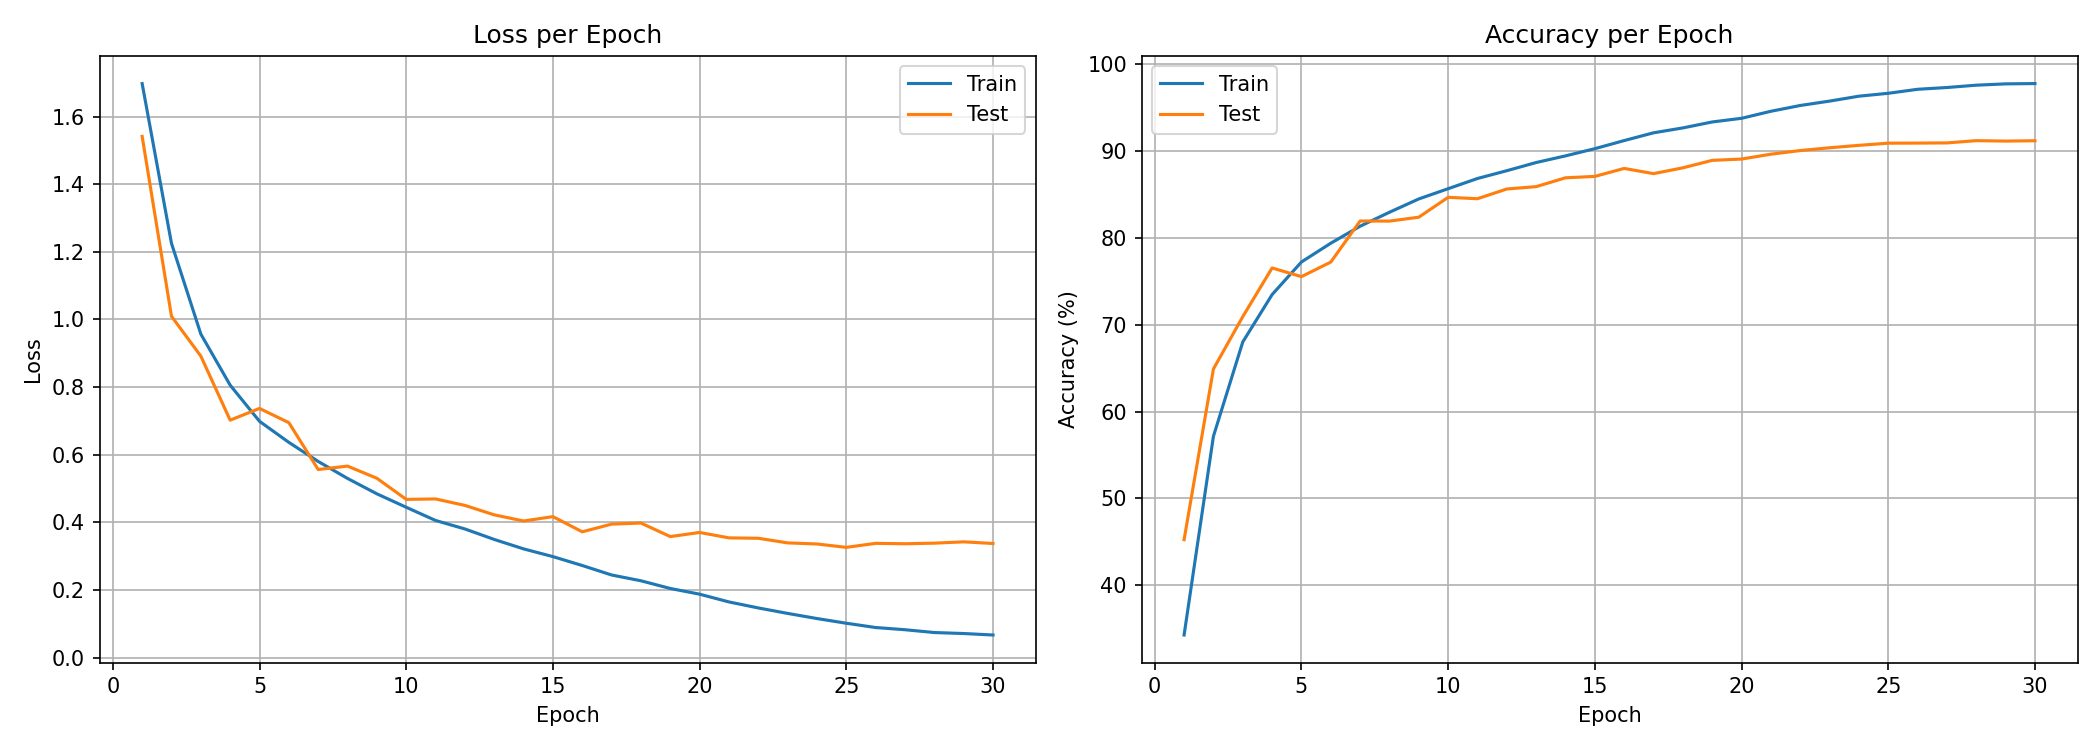
\includegraphics[width=0.95\linewidth]{training_curves.png}
    \caption{Training and test loss/accuracy curves for VGG19 on CIFAR-10.}
    \label{fig:curves}
\end{figure}

\section{Evaluation Metrics}

The best saved model was evaluated on the CIFAR-10 test set. Table~\ref{tab:overall_metrics} reports the main classification metrics. Since CIFAR-10 is balanced with 1,000 test samples per class, macro and weighted scores are almost identical.

\begin{table}[H]
\centering
\caption{Overall classification metrics on the CIFAR-10 test set.}
\label{tab:overall_metrics}
\begin{tabular}{lc}
\toprule
Metric & Value \\
\midrule
Accuracy & 91.22\% \\
Precision (macro) & 0.9122 \\
Recall (macro) & 0.9122 \\
F1-score (macro) & 0.9121 \\
Precision (weighted) & 0.9122 \\
Recall (weighted) & 0.9122 \\
F1-score (weighted) & 0.9121 \\
\bottomrule
\end{tabular}
\end{table}

Table~\ref{tab:class_metrics} shows the per-class precision, recall, and F1-score. The model performs best on car, ship, truck, frog, and horse classes. The most difficult classes are cat and dog, which is reasonable because these animal classes have similar visual patterns and larger intra-class variation.

\begin{table}[H]
\centering
\caption{Per-class classification report. Each class has 1,000 test samples.}
\label{tab:class_metrics}
\begin{tabular}{lcccc}
\toprule
Class & Precision & Recall & F1-score & Support \\
\midrule
Plane & 0.91 & 0.93 & 0.92 & 1000 \\
Car & 0.97 & 0.97 & 0.97 & 1000 \\
Bird & 0.89 & 0.87 & 0.88 & 1000 \\
Cat & 0.82 & 0.81 & 0.82 & 1000 \\
Deer & 0.88 & 0.92 & 0.90 & 1000 \\
Dog & 0.86 & 0.85 & 0.85 & 1000 \\
Frog & 0.95 & 0.94 & 0.94 & 1000 \\
Horse & 0.95 & 0.93 & 0.94 & 1000 \\
Ship & 0.95 & 0.95 & 0.95 & 1000 \\
Truck & 0.94 & 0.95 & 0.95 & 1000 \\
\bottomrule
\end{tabular}
\end{table}

The per-class accuracies are also high: plane 92.80\%, car 96.60\%, bird 87.20\%, cat 80.80\%, deer 91.70\%, dog 85.40\%, frog 94.30\%, horse 93.10\%, ship 94.80\%, and truck 95.50\%.

\section{Confusion Matrix and Sample Predictions}

Figure~\ref{fig:confusion} shows the confusion matrix. The diagonal values are dominant, which means most images are classified correctly. The largest confusions occur between visually similar classes, especially cat and dog. For example, 88 dog images are predicted as cat, and 81 cat images are predicted as dog. Some plane images are also confused with ship, and some car images are confused with truck.

\begin{figure}[H]
    \centering
    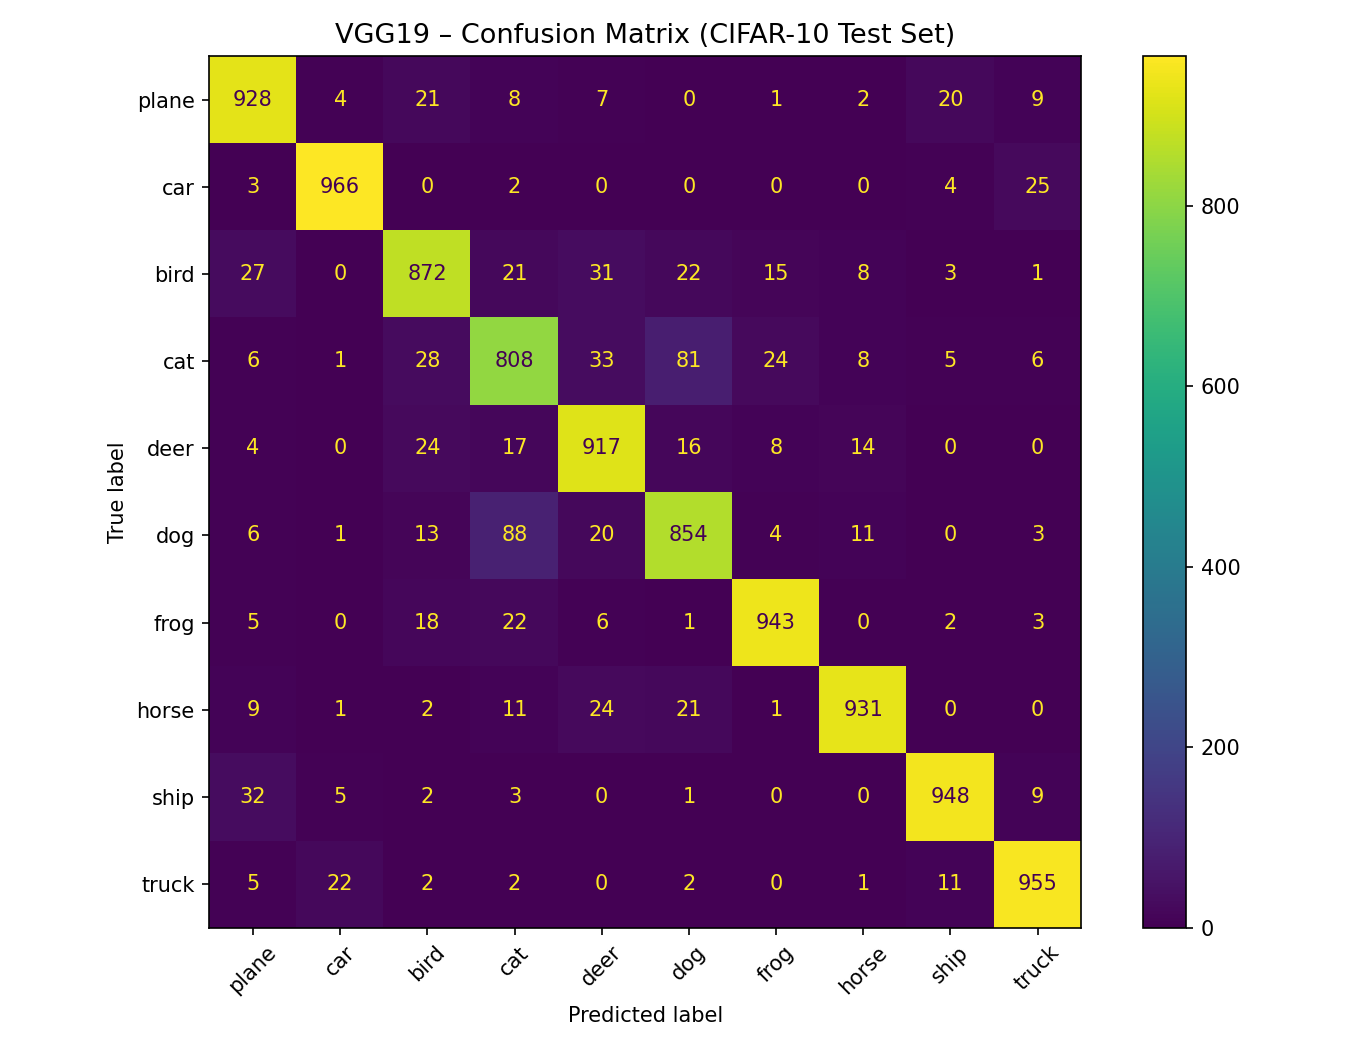
\includegraphics[width=0.72\linewidth]{vgg19_confusion_matrix.png}
    \caption{Confusion matrix of VGG19 on the CIFAR-10 test set.}
    \label{fig:confusion}
\end{figure}

Figure~\ref{fig:samples} shows several sample predictions. In the displayed batch, the predicted labels match the true labels, which visually confirms that the trained model can correctly recognize different object categories such as animals, vehicles, ships, and planes.

\begin{figure}[H]
    \centering
    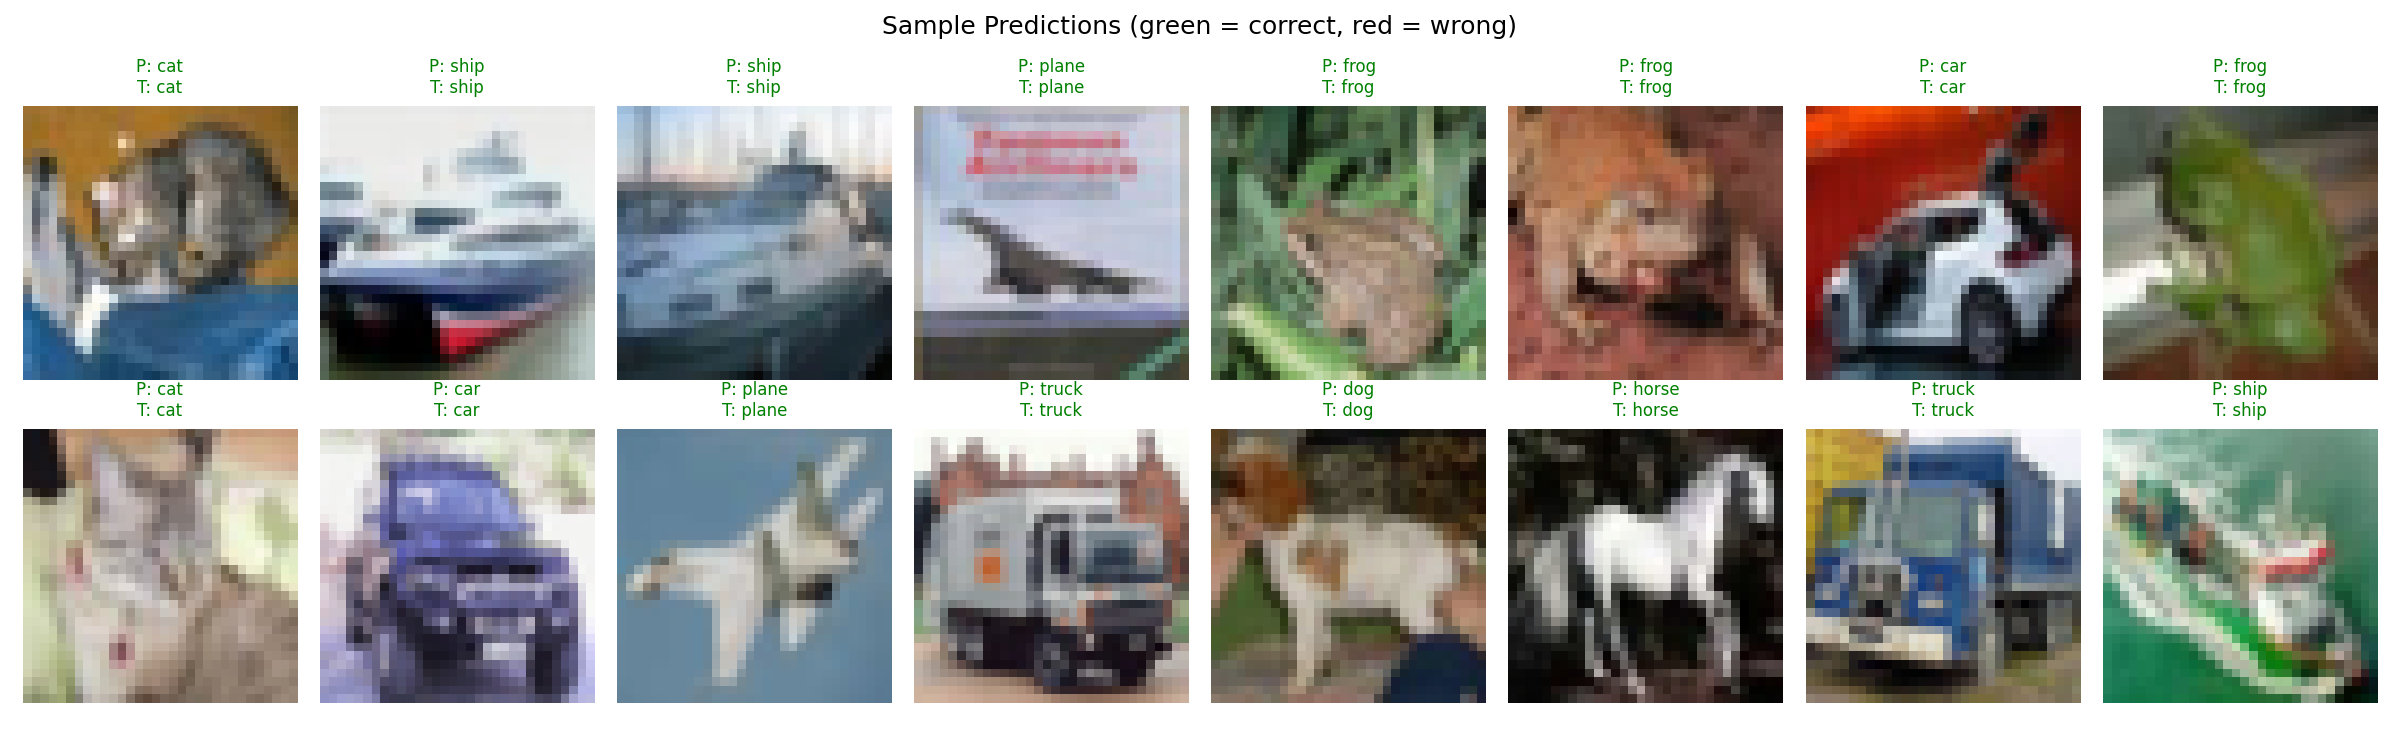
\includegraphics[width=0.98\linewidth]{sample_predictions.png}
    \caption{Sample predictions from the CIFAR-10 test set. Green labels indicate correct predictions.}
    \label{fig:samples}
\end{figure}

\section{Conclusion}

In this labwork, VGG19 was implemented from scratch in PyTorch and trained for CIFAR-10 image classification. The model achieved 91.22\% test accuracy, with macro precision 0.9122, macro recall 0.9122, and macro F1-score 0.9121. The results show that the VGG19 architecture can learn strong image features from CIFAR-10 without using pretrained weights. The main errors occur between visually similar classes, especially cat and dog, but the overall classification performance is high and stable.

\end{document}